\documentclass[18pt]{beamer}
\usepackage[utf8]{inputenc} % for the umlauts

\beamertemplatenavigationsymbolsempty
%% SLIDE FORMAT

% use 'beamerthemekit' for standard 4:3 ratio
% for widescreen slides (16:9), use 'beamerthemekitwide'

\usepackage{templates/beamerthemekit}
% \usepackage{templates/beamerthemekitwide}

\setcounter{tocdepth}{1}

%% TITLE PICTURE

% if a custom picture is to be used on the title page, copy it into the 'logos'
% directory, in the line below, replace 'mypicture' with the 
% filename (without extension) and uncomment the following line
% (picture proportions: 63 : 20 for standard, 169 : 40 for wide
% *.eps format if you use latex+dvips+ps2pdf, 
% *.jpg/*.png/*.pdf if you use pdflatex)

%\titleimage{mypicture}

%% TikZ INTEGRATION

% use these packages for PCM symbols and UML classes
% \usepackage{templates/tikzkit}
% \usepackage{templates/tikzuml}

% the presentation starts here

\title[SWT1]{Softwaretechnik 1 - 0. Tutorium}
\author{Felix Bachmann}

\institute{KIT - Institut für Programmstrukturen und Datenorganisation (IPD)}

% Bibliography

\usepackage[citestyle=authoryear,bibstyle=numeric,hyperref,backend=biber]{biblatex}
\addbibresource{templates/example.bib}
\bibhang1em

\begin{document}

% change the following line to "ngerman" for German style date and logos
\selectlanguage{ngerman}

%title page
\begin{frame}
\titlepage
\end{frame}

%table of contents
\begin{frame}{Themenübersicht}
\tableofcontents
\end{frame}

\section{Organisatorisches}
	\subsection{Vorstellung}
		\begin{frame}
			\frametitle{Das bin ich}
			\begin{itemize}
				\item Felix Bachmann
				\item Infostudent im 4. Semester
				\item erstes Tutorium
				\item E-Post-Adresse: felix.bachmann@ewetel.net
			\end{itemize}
		\end{frame}
		\begin{frame}
			\frametitle{\dots und ihr?}
			\begin{itemize}
				\item Name
				\item Studiengang und Semester
				\item erlernte Programmiersprachen, Lieblingsprogrammiersprache
				\item Erfahrung mit Git/Maven oder ähnlichen Tools?
				\item Von dem Tutorium erwarte ich\dots
			\end{itemize}
		\end{frame}
		
	\subsection{Regeln}
		\begin{frame}
			\frametitle{Verhalten im Tutorium}
			\begin{block}{cool}
				\begin{itemize}
					\item \textbf{mitdenken}
					\item \textbf{Fragen stellen}
					\item \textbf{Fragen beantworten}
					\item essen \& trinken
					\item gehen
					\item schlafen
				\end{itemize}
			\end{block}
			\pause
			\begin{block}{!cool}
				\begin{itemize}
					\item laut sein
					\item stören
					\item andere ablenken
				\end{itemize}
			\end{block}
		\end{frame}
		
	\subsection{Übungs- und Tutoriumsbetrieb}
		\begin{frame}
			\frametitle{Übungsbetrieb}
			\begin{itemize}
				\item Bestehen des Scheins Voraussetzung zum Bestehen des Moduls
				\item neue Übungsblätter ungefähr alle 2 Wochen $\implies$ 1+6 Blätter
				\item Übungen i.d.R. jeweils am Tag der Abgabe
				\item ab 50\% der Punkte habt ihr sicher bestanden
				\item Besprechung der Musterlösung
				\item Abgaben
					\begin{itemize}
						\item Theorieaufgaben+Deckblatt im 3.Stock
						\item Programmieraufgaben auf http://lez.ipd.kit.edu 
					\end{itemize}
			\end{itemize}
		\end{frame}
		
		\begin{frame}
			\frametitle{Tutoriumsbetrieb}
			\begin{itemize}
				\item Wann?: ab dem 15.05 14-tägig 
				\item Wo?: Raum -107
				\item Was?: 
					\begin{itemize}
						\item Wiederholung des VL-Stoffs
						\item "'Rechnen"' von Aufgaben (Altklausuren)
						\item ggf. Tipps für die Übungsblätter
					\end{itemize}
				\item Fragen stellen !!!
			\end{itemize}
		\end{frame}
		
	\subsection{Fragen}
		\begin{frame}
			\frametitle{Fragen zu Übung(sblättern), Vorlesung}
			erst im Forum, auf Google oder Stackoverflow nachschauen, dann
				\begin{itemize}
					\item neuen Forum-Thread anlegen
					\item falls nicht öffentlich postbar: Mail an mich oder swt1@ipd.kit.edu (nur im Notfall)
				\end{itemize}
		\end{frame}
		
\section{Vorbereitungsblatt}
	\begin{frame}
		\frametitle{Was ihr bisher getan haben solltet..}
		Installation von:
		\begin{itemize}
			\item Eclipse (incl. CheckStyle und EclEmma)
			\item Git
		\end{itemize}
		Überblick über:
		\begin{itemize}
			\item Maven
			\item Git
		\end{itemize}
		Probleme mit der Installation? $\implies$ kommt nach dem Tut nach vorne
	\end{frame}
		
		
\section{JUnit4}	
	\begin{frame}
		\frametitle{JUnit4 - Überblick}
		\begin{itemize}
			\item Test-Tool für Java-Klassen
			\item Nur öffentliche Methoden testen
			\item Konventionen:
			 \begin{itemize}
			 		\item Für Klasse Hallo Testklasse HalloTest schreiben
			 		\item Methode hallo(Object o) wird z.B. durch die Methode testHalloWithNull() getestet
			 \end{itemize}
		\end{itemize}
	\end{frame}	
	
	\begin{frame}
		\frametitle{JUnit4 - Aufbau einer Testklasse}
		Methoden können mit Annotationen (@XYZ) versehen werden \linebreak
		Aufbau:
		\begin{itemize}
			\item @BeforeClass (wird als erstes einmal ausgeführt)
			\pause
			\item @Before (wird vor jeder Test-Methode einmal ausgeführt)
			\pause
			\item @Test (vergleichen erwartetes und reales Ergebnis, schlagen ggf. fehl, Ausführung in beliebiger Reihenfolge)
			\pause
			\item @After (wird nach jeder Test-Methode einmal ausgeführt)
			\pause
			\item @AfterClass (wird am ende einmal ausgeführt)
		\end{itemize}
	\end{frame}
	
	\begin{frame}
		\frametitle{JUnit4 - Assert}
		org.junit.Assert bietet diverse Methoden, um Ergebnis mit Erwartung abzugleichen \linebreak
		zu jeder Methode kann als erstes Argument ein String mitgegeben werden (wird bei Fehlschlag angezeigt) \linebreak
		Beispiele:
		\begin{itemize}
			\item assertArrayEquals(int[] expected, int[] actual)
			\item assertNotNull(Object obj)
			\item assertSame(Object expected, Object actual)
		\end{itemize}
	\end{frame}
	
	\begin{frame}
		\frametitle{JUnit4 - eine Testmethode}
		\begin{block}{Zu testende Methode in der Klasse Hallo}
				public static int add(int a, int b) \{ \linebreak
					 return a + b; \linebreak
				      \}	
		\end{block} 
		\begin{block}{Testmethode in der Klasse HalloTest}
			@Test\linebreak
			public void testAdd() \{ \linebreak
				Assert.assertEquals(7, Hallo.add(5 + 2)); \linebreak
			\}
		\end{block}
		(mehr Beispiele später)
	\end{frame}
		
\section{Maven}
	\begin{frame}
		\frametitle{Maven - Überblick}
		\begin{itemize}
			\item Maven ist in jeder Eclipse-Installation integriert \linebreak $\implies$ keine manuelle Installation nötig
			\item Aufgaben von Maven
				\begin{itemize}
					\item Strukturierung (durch vorgegebene Verzeichnisstruktur)
					\item Kompilieren
					\item Testen
					\item Verwalten von Abhängigkeiten
					\item Verpacken
				\end{itemize}
		\end{itemize}
	\end{frame}
	
	\begin{frame}
		\frametitle{Maven - Überblick}
		Verzeichnisstruktur:
	\end{frame}
	
	\begin{frame}
		\frametitle{Maven - Überblick}
		\begin{block}{Wichtige Befehle}
			\begin{tabular}{ll}
				\texttt{mvn compile} & kompiliert Quelltexte zu .class-Dateien \\
				\texttt{mvn test} & kompiliert Test-Quelldateien zu .class-Dateien, \\ & führt Tests aus und zeigt Ergebnisse an \\
				\texttt{mvn package} & verpackt euer Projekt in eine Datei (.war/.jar/.zip) \\ 
				\texttt{mvn clear} & leert euren target-Ordner \\
			\end{tabular}
		\end{block}
	\end{frame}


		
		
\section{Tipps}
%TODO Reminder Abgabe
		

		\begin{frame}
			\frametitle{Bis dann! (dann=15.05.17)}
			\centering
			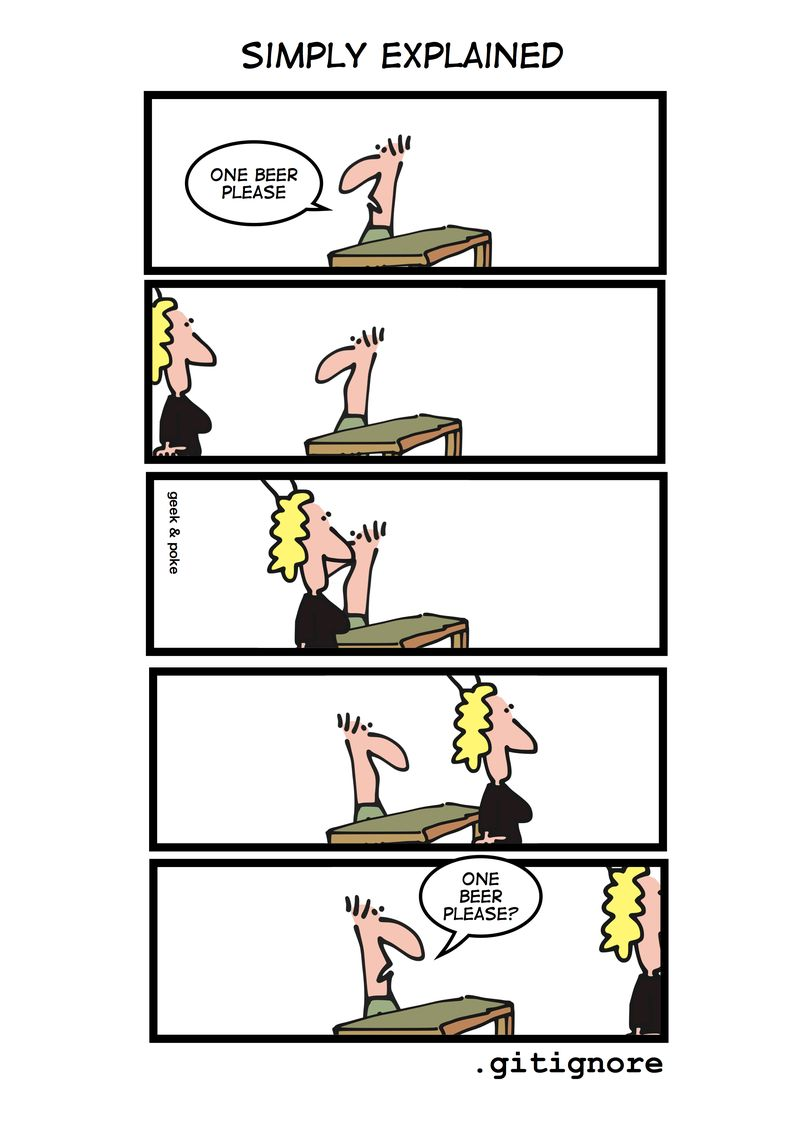
\includegraphics[height=0.85\textheight]{./comics/geek_and_poke_gitignore.jpg}
			\tiny\url{geek-and-poke.com/geekandpoke/2012/11/7/simply-explained.html}
		\end{frame}

\end{document}
